% =====================================================================
%  NOISE -- prehľadový článok (predbežná verzia)
%  Metódy inžinierskej práce 2026/27, FIIT STU
%  Preklad: pdflatex clanok; bibtex clanok; pdflatex clanok; pdflatex clanok
% =====================================================================
\documentclass[10pt,twoside,a4paper]{article}

\usepackage[T1]{fontenc}
\usepackage[utf8]{inputenc}
\usepackage[provide=*,slovak]{babel}
\usepackage{mathptmx}
\usepackage{courier}
\usepackage{graphicx}
\usepackage{booktabs,tabularx}
\usepackage{xcolor}
\usepackage{url}
\usepackage[hidelinks]{hyperref}
\usepackage{cite}

\setlength{\emergencystretch}{2em}
\newcommand{\doplnit}[1]{\textcolor{red}{[#1]}}
\newcommand{\mb}{$\bullet$}

\pagestyle{headings}

\title{Nevizuálne snímanie obsadenosti uzavretých priestorov: prehľad metód s~ohľadom na ochranu súkromia a~odolnosť v~kritických podmienkach\thanks{Semestrálny projekt v~predmete Metódy inžinierskej práce, ak. rok 2026/27, vedenie: \doplnit{meno cvičiaceho}}}

\author{Oliver Pribula \and Lukáš Poláček \and Martin Pivko \and Daniil Romashov\\[6pt]
{\small Slovenská technická univerzita v~Bratislave}\\
{\small Fakulta informatiky a~informačných technológií}\\
{\small \texttt{\doplnit{xlogin}@stuba.sk}}}

\date{\small 26. októbra 2026}

\begin{document}

\maketitle

\begin{abstract}
Údaj o~tom, koľko ľudí sa nachádza v~miestnosti, potrebujú správcovia budov na riadenie vykurovania a~vetrania, prevádzkovatelia služieb na informovanie zákazníkov a~záchranné zložky pri požiari. Najrozšírenejším zdrojom tohto údaja sú kamery, ktoré však zaznamenávajú identitu osôb a~v~tme či v~dyme zlyhávajú. Článok prináša prehľad nevizuálnych metód zisťovania obsadenosti -- environmentálnych senzorov, nízkorozlíšených termálnych polí, snímania pomocou Wi-Fi, radarov v~pásme milimetrových vĺn a~aktívneho akustického snímania -- a~porovnáva ich z~hľadiska presnosti odhadu počtu osôb, ochrany súkromia, odolnosti v~zhoršených podmienkach a~ceny. Prehľad vychádza z~rešerše v~databázach IEEE Xplore a~Web of Science za roky 2018--2026. Ukazujeme, že žiadna z~modalít sama nespĺňa všetky požiadavky a~že absencia kamery ešte nezaručuje anonymitu: rádiové signály aj nízkorozlíšené termálne obrazy nesú biometrické vzory a~rádiový kanál môže odpočúvať aj tretia strana. Na základe prehľadu navrhujeme koncept systému NOISE, ktorý kombinuje rádiofrekvenčné a~termálne snímanie s~adaptívnym váhovaním modalít a~spracúva údaje výlučne priamo v~zariadení. Záver článku sumarizuje otvorené problémy, ktorými sa bude projekt ďalej zaoberať.
\end{abstract}

% ---------------------------------------------------------------------
\section{Úvod}\label{uvod}

Obsadenosť priestoru, teda informácia o~tom, či a~koľko ľudí sa v~ňom nachádza, je vstupom pre množstvo rozhodnutí. V~budovách podľa nej možno riadiť vykurovanie, vetranie a~klimatizáciu tak, aby sa neplytvalo energiou v~prázdnych miestnostiach a~aby v~plných miestnostiach nebolo vydýchané~\cite{amiri2025review}. Prevádzkovatelia fitness centier, knižníc či reštaurácií ju môžu zobrazovať zákazníkom. V~krízovej situácii, napríklad pri požiari, je rovnaký údaj otázkou života: veliteľ zásahu potrebuje vedieť, či a~kde zostali v~budove ľudia.

Súčasné riešenia majú dve skupiny nedostatkov. Kamerové systémy dokážu ľudí spočítať presne, ale zaznamenávajú ich identitu. Ich nasadenie v~kanceláriách, šatniach alebo ubytovacích priestoroch naráža na legislatívu o~ochrane osobných údajov~\cite{gdpr2016} aj na odpor samotných ľudí. Navyše optické snímanie prestáva fungovať práve v~situáciách, keď je údaj najcennejší -- v~tme a~v~dyme. Druhú skupinu tvoria riešenia vyžadujúce spoluprácu ľudí, napríklad registrácia pri vstupe alebo mobilná aplikácia. Tie poskytujú neúplné údaje, lebo ich ľudia nepoužívajú dôsledne, a~v~kríze sú nepoužiteľné.

Tento článok sa zaoberá otázkou, či sa dá počet osôb v~uzavretej miestnosti spoľahlivo zistiť bez toho, aby sme ich videli. K~téme nás primárne usmernil prehľad systémov merania obsadenosti budov od Suna a~kol.~\cite{sun2020review}, ktorý triedi existujúce prístupy podľa typu senzora a~upozorňuje na napätie medzi presnosťou a~ochranou súkromia. Oproti nemu kladieme dôraz na dve požiadavky, ktoré sa v~literatúre riešia oddelene: anonymitu v~bežnej prevádzke a~funkčnosť v~kritických podmienkach.

Článok je organizovaný nasledovne. V~časti~\ref{poziadavky} definujeme úlohu, požiadavky na jej riešenie a~postup rešerše. Časť~\ref{prehlad} prináša prehľad nevizuálnych modalít a~časť~\ref{porovnanie} ich porovnanie spolu s~prehľadom prístupov k~fúzii. V~časti~\ref{sukromie} ukazujeme, prečo nevizuálne snímanie automaticky neznamená anonymitu. Časť~\ref{kriticke} sa venuje správaniu senzorov v~dyme a~pri požiari. V~časti~\ref{noise} opisujeme koncept systému NOISE, ktorý z~prehľadu vychádza. Časť~\ref{zaver} uzatvára článok a~sumarizuje otvorené problémy.

% ---------------------------------------------------------------------
\section{Úloha, požiadavky a~postup rešerše}\label{poziadavky}

V~literatúre sa pod pojmom obsadenosť rozumejú úlohy rôznej náročnosti~\cite{chen2018review,sun2020review}. Najjednoduchšou je \emph{detekcia prítomnosti}, teda rozhodnutie, či je miestnosť prázdna. Náročnejší je \emph{odhad počtu} osôb a~najnáročnejšia je \emph{lokalizácia}, teda určenie, kde sa osoby nachádzajú, prípadne sledovanie ich pohybu. Pre riadenie budovy často postačí prítomnosť alebo hrubý počet, pre zobrazenie vyťaženosti služby je potrebný počet a~pre záchranárov je užitočná aj približná poloha.

Pre účely tohto prehľadu hodnotíme metódy podľa štyroch kritérií:
\begin{enumerate}
\item \textbf{Presnosť odhadu počtu} -- či metóda dokáže rozlíšiť počet osôb, nielen prítomnosť, a~ako sa jej presnosť mení s~rastúcim počtom osôb.
\item \textbf{Ochrana súkromia} -- či z~údajov, ktoré metóda zaznamenáva, možno identifikovať konkrétnu osobu alebo odvodiť citlivé informácie o~nej.
\item \textbf{Odolnosť v~zhoršených podmienkach} -- či metóda funguje v~tme, v~dyme a~pri zvýšenej teplote.
\item \textbf{Cena a~nasaditeľnosť} -- cena hardvéru, nároky na inštaláciu a~kalibráciu v~novej miestnosti.
\end{enumerate}

Dôležitou implicitnou požiadavkou je, aby metóda nevyžadovala \emph{spoluprácu} osôb, teda aby nemuseli nosiť žiadne zariadenie ani vykonávať žiadnu akciu. Takéto snímanie sa označuje ako bezkontaktné alebo bez zariadenia (angl.~\emph{device-free}).

\paragraph{Postup rešerše.} Okrem primárneho zdroja~\cite{sun2020review} a~starších základných prác sme literatúru vyhľadávali v~databázach IEEE Xplore a~Web of Science Core Collection s~obmedzením na roky 2018--2026. Dopyty pokrývali šesť okruhov: odhad počtu osôb pomocou CSI, radaru a~termálnych polí; fúziu modalít; detekciu osôb v~dyme a~pri záchranných akciách; súkromie a~identifikáciu osôb z~rádiových signálov; akustické snímanie; a~spracovanie na mikrokontroléroch. Z~792 exportovaných záznamov zostalo po odstránení duplikátov medzi databázami 682. Na základe názvov a~abstraktov sme vylúčili práce mimo uzavretých priestorov (parkoviská, drony, kabíny vozidiel) a~práce založené na kamerách a~z~ostatných sme vybrali tie, ktoré uvádzajú experimentálne overenie alebo súhrnný pohľad na niektoré z~našich kritérií. Číselné výsledky citovaných prác preberáme z~ich abstraktov; boli namerané v~rôznych podmienkach, preto ich nemožno priamo porovnávať.

% ---------------------------------------------------------------------
\section{Prehľad nevizuálnych modalít}\label{prehlad}

\subsection{Environmentálne a~pohybové senzory}

Najlacnejšou skupinou sú senzory, ktoré sú v~budovách často už nainštalované. Pasívne infračervené (PIR) senzory pohybu reagujú na zmenu tepelného žiarenia v~zornom poli, preto spoľahlivo zachytia vstup osoby do miestnosti, no nezachytia osobu, ktorá sedí alebo leží bez pohybu. Počet osôb z~nich priamo zistiť nemožno~\cite{sun2020review}.

Koncentrácia oxidu uhličitého v~miestnosti rastie s~počtom osôb, ktoré dýchajú. Jin a~kol.~\cite{jin2018occupancy} ukázali, že s~využitím fyzikálneho modelu šírenia CO\textsubscript{2} vo vetranej miestnosti možno obsadenosť odhadovať presnejšie než čisto štatistickými metódami. Chitnis a~kol.~\cite{chitnis2025environmental} však na verejnom súbore údajov z~kancelárskej budovy dosiahli z~CO\textsubscript{2}, teploty a~vlhkosti presnosť detekcie prítomnosti len 66--82\,\% a~presnosť odhadu úrovne či počtu 69--80\,\%; modely založené na jedinom environmentálnom senzore pritom zaostávali za kombináciou senzorov. Princíp má aj prirodzené obmedzenia: koncentrácia sa mení pomaly, závisí od vetrania a~otvárania okien a~v~priestore zasiahnutom požiarom je CO\textsubscript{2} produktom horenia, takže prestáva niesť informáciu o~ľuďoch. Environmentálne senzory sú teda vhodné ako doplnkový zdroj, nie ako jediný.

\subsection{Nízkorozlíšené termálne polia}

Termálne polia (angl.~\emph{thermopile array}) merajú teplotu v~mriežke s~nízkym rozlíšením, typicky 8$\times$8 až 32$\times$24 bodov. Ľudské telo sa v~takom obraze prejaví ako škvrna vyššej teploty, ale tvár ani postava nie sú rozpoznateľné. Beltran a~kol.~\cite{beltran2013thermosense} v~systéme ThermoSense spojili termálne pole 8$\times$8 so senzorom pohybu a~odhadovali počet osôb na účely riadenia vykurovania a~klimatizácie. Výhodou je, že senzor zachytí aj nehybnú osobu a~spracovanie je výpočtovo nenáročné. Rinta-Homi a~kol.~\cite{rintahomi2021howlow} systematicky skúmali, ako nízko možno ísť s~rozlíšením: spoľahlivú detekciu prítomnosti dosiahli už pri rozlíšení 4$\times$2 bodov, ak snímková frekvencia neklesla pod 4~snímky za sekundu, a~výsledky boli citlivé na uhol pohľadu senzora. Nižšie rozlíšenie pritom znamená menej informácie o~identite osôb aj nižšiu cenu.

Obmedzenia vyplývajú z~fyzikálneho princípu. Termálne pole meria rozdiel teplôt medzi človekom a~pozadím; keď sa teplota okolia priblíži k~teplote povrchu tela, kontrast zaniká. Prekážkou sú aj iné zdroje tepla (radiátory, notebooky, horúce nápoje) a~vzájomné zakrývanie osôb, keď sa dve škvrny spoja do jednej. Papanashi a~kol.~\cite{papanashi2026thermal} statické zdroje tepla odlišujú od ľudí podľa toho, či škvrna v~čase vykazuje mikropohyby, a~celé spracovanie vrátane sledovania osôb vykonávajú na mikrokontroléri ESP32 s~520~kB SRAM. Risso a~kol.~\cite{risso2024hwsw} ukázali, že automatizovaným návrhom architektúry neurónovej siete a~kvantizáciou možno počítanie osôb z~infračerveného poľa na mikrokontroléri zrýchliť a~zúsporniť, pri rovnakej presnosti až 15-násobne nižšou spotrebou energie.

\subsection{Snímanie pomocou Wi-Fi}

Ľudské telo pozostáva prevažne z~vody, preto ovplyvňuje šírenie rádiových vĺn: tieni priamu cestu medzi vysielačom a~prijímačom a~vytvára nové odrazy. Wi-Fi snímanie využíva túto vlastnosť a~nevyžaduje žiadny špeciálny vysielač -- postačuje komunikácia bežných zariadení~\cite{shahbazian2023survey}.

Najjednoduchšou veličinou je intenzita prijímaného signálu (RSSI). Depatla a~kol.~\cite{depatla2015occupancy} ukázali, že už z~meraní intenzity medzi jedným párom vysielača a~prijímača možno odhadnúť počet osôb, ak sa vhodne modeluje tienenie priamej cesty a~rozptyl signálu na ľuďoch. Bohatšiu informáciu poskytuje kanálová informácia (angl.~\emph{Channel State Information}, CSI), ktorá opisuje amplitúdu a~fázu signálu na každej z~podnosných frekvencií. Ma a~kol.~\cite{ma2019wifi} v~prehľade opisujú, ako sa CSI využíva na detekciu prítomnosti, rozpoznávanie aktivít aj odhad počtu osôb, a~zhŕňajú typický reťazec spracovania: odstránenie šumu, extrakciu príznakov a~klasifikáciu. Xi a~kol.~\cite{xi2014frog} využili pozorovanie, že variabilita CSI rastie s~počtom pohybujúcich sa osôb, a~na tomto princípe navrhli metódu počítania davu. Zou a~kol.~\cite{zou2018wifree} v~systéme WiFree získavali CSI priamo z~bežných smerovačov a~v~troch miestnostiach rôznej veľkosti uvádzajú presnosť 99,1\,\% pri detekcii prítomnosti a~92,8\,\% pri odhade počtu osôb.

Väčšina metód stavia na pohybe, ktorý mení kanál. Sediaci ľudia sa však tiež nehýbu úplne: Korany a~Mostofi~\cite{korany2021stationary} ukázali, že drobné pohyby pri sedení (posunutie sa na stoličke, prekríženie nôh) nesú informáciu o~počte osôb, a~ich štatistickým modelom odhadli počet až 10~sediacich ľudí s~chybou najviac jednej osoby v~96,3\,\% prípadov, cez stenu v~90\,\% prípadov.

Hlavným problémom Wi-Fi snímania je závislosť od prostredia. Model naučený v~jednej miestnosti nemusí fungovať v~inej, ba ani v~tej istej po presunutí nábytku, pretože sa zmení viaccestné šírenie signálu~\cite{ma2019wifi}. Santos a~kol.~\cite{santos2024environment} zbierali CSI tri mesiace v~rôznych miestnostiach a~model natrénovaný bez údajov z~cieľového prostredia v~ňom fungoval zreteľne horšie; doplnenie časti údajov z~cieľového prostredia zvýšilo presnosť klasifikácie približne o~16--20\,\%. Na zníženie kalibrácie sa preto skúma učenie z~malého počtu príkladov: metóda DASECount~\cite{hou2023dasecount} sa prispôsobí novému prostrediu už z~piatich označených vzoriek na triedu a~pri počítaní 0--8~osôb uvádza priemernú presnosť 96,4\,\%. Signál tiež ovplyvňujú susedné siete a~ľudia za stenou.

\subsection{Radary v~pásme milimetrových vĺn}

Radary s~frekvenčne modulovanou nosnou vlnou (FMCW) merajú vzdialenosť, rýchlosť a~uhol odrazených objektov. V~pásme 60--80~GHz, teda pri vlnových dĺžkach okolo 4--5~mm, dosahujú rozlíšenie v~rádoch centimetrov a~sú komerčne dostupné ako lacné jednočipové moduly. Zhao a~kol.~\cite{zhao2019mid} použili radar v~tomto pásme na súčasné sledovanie viacerých osôb v~miestnosti. Rádiové snímanie zachytí aj veľmi jemné pohyby: Adib a~kol.~\cite{adib2015vital} merali FMCW rádiom dýchanie a~tep viacerých ľudí naraz bez akéhokoľvek kontaktu. Pre úlohu obsadenosti je to podstatné, lebo vďaka tomu možno odlíšiť nehybného človeka od predmetu -- človek dýcha. Tento princíp využili Weiss a~kol.~\cite{weiss2020people}: kandidátov na osoby nájdených v~spektre vzdialeností overovali podľa prítomnosti vitálnych funkcií a~s~radarom 60~GHz dosiahli v~kancelárii s~0--4~osobami presnosť $\pm 1$~osoba v~85,4\,\% prípadov. Systém MMCOUNT~\cite{hu2024mmcount} kombinuje dýchanie a~drobné pohyby a~v~posluchárni, triede aj zasadačke počítal sediace osoby s~presnosťou až 95,8\,\%, a~to aj pri vzájomnej vzdialenosti osôb 0,4~m.

Radar je oproti Wi-Fi menej závislý od usporiadania miestnosti, pretože meria priamo polohu odrazov. Jeho dosah je však obmedzený zorným poľom antény a~pri väčšom počte blízko stojacich ľudí sa odrazy prekrývajú. Ren a~kol.~\cite{ren2023grouped} sa zaoberali práve skupinami osôb, ktoré sú bližšie pri sebe, než je rozlišovacia schopnosť radaru, a~kombinovali sledovanie skupiny s~klasifikátorom počtu osôb v~nej. Ani radar nie je úplne nezávislý od prostredia: modely naučené pri jednom usporiadaní odrazov od okolitých predmetov sa podobne ako pri Wi-Fi musia prispôsobovať novým miestnostiam. Výpočtová náročnosť naopak prekážkou nie je -- Mach a~kol.~\cite{mach2024uwb} spustili kvantizovanú konvolučnú sieť na počítanie až 10~osôb z~ultraširokopásmového radaru na mikrokontroléroch STM32 s~časom inferencie pod 48~ms.

\subsection{Akustické snímanie}

Aktívne akustické snímanie vysiela zvukový signál v~nepočuteľnom pásme a~vyhodnocuje jeho odrazy, podobne ako sonar. Nandakumar a~kol.~\cite{nandakumar2015apnea} ukázali, že už bežný smartfón dokáže z~odrazov nepočuteľného signálu vyslaného reproduktorom sledovať dýchacie pohyby spiaceho človeka. Altinses a~Schwung~\cite{altinses2026sonar} použili aktívny sonar priamo na odhad obsadenosti miestnosti s~argumentom, že optické senzory v~dyme zlyhávajú; ich model kombinuje Sabinovu teóriu dozvuku s~neurónovou sieťou a~v~troch prostrediach dosiahol presnosť detekcie 84,5\,\%. Výhodou je nízka cena reproduktora a~mikrofónov. Pre počítanie osôb v~celej miestnosti je však akustické snímanie citlivé na hluk a~ozvenu a~mikrofón v~zariadení vyvoláva obavy o~súkromie. Tie sú opodstatnené: Williams a~kol.~\cite{williams2023audio} odhadovali počet hovoriacich osôb z~pasívne zaznamenaného zvuku a~ani po náhodnom narušení zvukových rámcov, ktoré skrylo obsah reči, nedokázali úplne zabrániť rozpoznaniu hovoriacich. Túto modalitu v~projekte považujeme za doplnkovú, v~aktívnom režime bez záznamu reči, a~jej prínos ešte overíme.

% ---------------------------------------------------------------------
\section{Porovnanie modalít}\label{porovnanie}

Tabuľka~\ref{tab:porovnanie} zhŕňa porovnanie modalít podľa kritérií z~časti~\ref{poziadavky}. Hodnotenie je kvalitatívne a~vychádza z~prehľadov~\cite{sun2020review,chen2018review,ma2019wifi,shahbazian2023survey}, z~prác uvedených v~časti~\ref{prehlad} a~z~fyzikálnych princípov. Kameru uvádzame ako referenciu. Tabuľka~\ref{tab:vysledky} dopĺňa vybrané kvantitatívne výsledky z~rešerše.

\begin{table}[ht]
\centering
\caption{Kvalitatívne porovnanie modalít (\mb\mb\mb{} = najlepšie)}\label{tab:porovnanie}
\small
\begin{tabular}{@{}lcccc@{}}
\toprule
Modalita & Odhad počtu & Súkromie & Tma a~dym & Nízka cena \\
\midrule
Kamera (optická)      & \mb\mb\mb & \mb       & \mb       & \mb\mb    \\
PIR senzor pohybu     & \mb       & \mb\mb\mb & \mb\mb    & \mb\mb\mb \\
Senzor CO\textsubscript{2} & \mb  & \mb\mb\mb & \mb       & \mb\mb    \\
Termálne pole         & \mb\mb    & \mb\mb\mb & \mb\mb    & \mb\mb    \\
Wi-Fi CSI             & \mb\mb    & \mb\mb    & \mb\mb\mb & \mb\mb\mb \\
mmWave radar          & \mb\mb\mb & \mb\mb    & \mb\mb\mb & \mb\mb    \\
Akustické snímanie    & \mb\mb    & \mb       & \mb\mb\mb & \mb\mb\mb \\
\bottomrule
\end{tabular}
\end{table}

\begin{table*}[t]
\centering
\caption{Vybrané výsledky z~rešerše (údaje z~abstraktov; podmienky meraní sa líšia, hodnoty nie sú priamo porovnateľné)}\label{tab:vysledky}
\small
\begin{tabularx}{\textwidth}{@{}llX@{}}
\toprule
Práca & Modalita & Úloha a~uvádzaný výsledok \\
\midrule
WiFree~\cite{zou2018wifree} & Wi-Fi CSI & počet osôb v~3~miestnostiach, presnosť 92,8\,\% \\
Korany a~Mostofi~\cite{korany2021stationary} & Wi-Fi CSI & až 10 sediacich osôb, chyba $\le 1$ v~96,3\,\% (cez stenu 90\,\%) \\
DASECount~\cite{hou2023dasecount} & Wi-Fi CSI & 0--8~osôb v~novom prostredí z~5~vzoriek na triedu, priemerne 96,4\,\% \\
Weiss a~kol.~\cite{weiss2020people} & radar 60~GHz & 0--4~osoby, overenie vitálnych funkcií, $\pm 1$ v~85,4\,\% \\
MMCOUNT~\cite{hu2024mmcount} & mmWave radar & sediace osoby, presnosť do 95,8\,\% \\
Mach a~kol.~\cite{mach2024uwb} & UWB radar & do 10~osôb, 98,2\,\% po kvantizácii, MCU STM32 \\
Rinta-Homi a~kol.~\cite{rintahomi2021howlow} & termálne pole & prítomnosť spoľahlivo už pri 4$\times$2~bodoch a~$\ge 4$~snímkach/s \\
Papanashi a~kol.~\cite{papanashi2026thermal} & termálne pole & počet a~sledovanie osôb celé na ESP32 (520~kB SRAM) \\
Altinses a~Schwung~\cite{altinses2026sonar} & aktívny sonar & obsadenosť v~3~prostrediach, presnosť 84,5\,\% \\
Chitnis a~kol.~\cite{chitnis2025environmental} & CO\textsubscript{2}, teplota, vlhkosť & prítomnosť 66--82\,\%, úroveň alebo počet 69--80\,\% \\
\bottomrule
\end{tabularx}
\end{table*}

Z~porovnania vyplývajú dve pozorovania. Po prvé, žiadna modalita nedosahuje najlepšie hodnotenie vo všetkých kritériách. Rádiové metódy sú najodolnejšie voči zhoršenej viditeľnosti, termálne pole má najlepšiu vrodenú anonymitu (s~výhradou uvedenou v~časti~\ref{sukromie}) a~environmentálne senzory sú najlacnejšie, ale najmenej presné. Po druhé, slabiny jednotlivých modalít sa nekryjú: termálne pole zlyháva pri vysokej teplote, keď rádiové snímanie funguje ďalej, a~Wi-Fi zlyháva pri rádiovom rušení, ktoré termálne pole neovplyvní. To naznačuje, že vhodná kombinácia modalít môže prekonať každú z~nich samostatne.

\paragraph{Fúzia modalít.} Literatúra túto domnienku podporuje, hoci väčšinou pri iných kombináciách senzorov, než aké uvažujeme my. Hobson a~kol.~\cite{hobson2019opportunistic} spájali v~kancelárskej budove údaje, ktoré už existovali -- počty zariadení pripojených k~Wi-Fi, CO\textsubscript{2}, PIR a~spotrebu elektriny -- a~samotné počty Wi-Fi zariadení vysvetľovali počas obsadených hodín 80--83\,\% rozptylu skutočného počtu osôb. Rafi a~kol.~\cite{rafi2024dwfl} navrhli fúziu, ktorá každému senzoru priraďuje váhu podľa podmienok v~miestnosti, a~uvádzajú presnosť odhadu počtu 94\,\%, o~3~percentuálne body viac než porovnávané metódy. Cui a~Zheng~\cite{cui2026em2} riešili opačný problém, energetickú náročnosť: ich rámec E-M2 počas behu vypína modality, ktoré v~danej chvíli neprinášajú novú informáciu, a~príležitostne ich opäť zapína, čím znížil spotrebu v~priemere o~40,8\,\% bez straty presnosti. Prácu, ktorá by na počítanie osôb v~budove spájala práve rádiové a~termálne senzory s~váhami odvodenými od kvality signálu, sme v~prehľadaných záznamoch nenašli; najbližšie k~nej majú práce o~detekcii osôb v~dyme (časť~\ref{kriticke}).

% ---------------------------------------------------------------------
\section{Nevizuálne neznamená anonymné}\label{sukromie}

Bežný argument v~prospech nevizuálnych senzorov je, že nezaznamenávajú tvár, a~teda chránia súkromie. Tento argument je však neúplný. Nariadenie GDPR~\cite{gdpr2016} sa nevzťahuje len na fotografie, ale na akékoľvek údaje, z~ktorých možno fyzickú osobu identifikovať, a~osobitne chráni biometrické a~zdravotné údaje.

Viaceré práce ukazujú, že rádiové signály takúto informáciu nesú. Wang a~kol.~\cite{wang2016gait} rozpoznávali ľudí podľa chôdze len z~CSI bežnej Wi-Fi siete. Zhao a~kol.~\cite{zhao2019mid} pomocou mmWave radaru osoby nielen sledovali, ale aj rozlišovali, kto je kto, na základe tvaru ich odrazov. Systém MU-ID~\cite{yang2020muid} s~jedným komerčným radarom identifikoval jednu osobu podľa chôdze s~presnosťou až 97\,\% a~až štyri súčasne kráčajúce osoby s~presnosťou nad 92\,\%. Gonzalez a~kol.~\cite{gonzalez2025informer} z~radarových mračien bodov počas chôdze odhadovali výšku, hmotnosť, pohlavie aj obvod pása, s~presnosťou do 82\,\%. Systém Vital-Radio~\cite{adib2015vital} meria dýchanie a~tep, teda údaje, ktoré majú zdravotný charakter. Ani termálne polia nie sú voči identifikácii imúnne: Jiang a~kol.~\cite{jiang2026warmgait} z~lacných termálnych polí rozpoznávali osoby podľa chôdze s~priemernou presnosťou 87,3\,\%. Z~toho vyplýva, že ochranu súkromia nemožno odvodiť len od typu senzora; záleží aj od rozlíšenia a~od toho, čo sa so surovými údajmi deje~\cite{rintahomi2021howlow}.

Za kľúčové preto považujeme \emph{miesto spracovania}. Ak surové signály opustia senzor a~ukladajú sa na server, vzniká databáza, z~ktorej by sa dali identifikačné vzory dodatočne vyťažiť. Ak sa naopak všetko spracuje priamo v~zariadení a~von odchádza iba agregovaný údaj -- počet osôb -- identifikácia je obmedzená samotnou architektúrou. Výpočet na hrane, teda priamo na mikrokontroléri senzora, je dnes realistický: rámce ako TensorFlow Lite Micro~\cite{david2021tflm} umožňujú spúšťať kvantizované neurónové siete na zariadeniach s~pamäťou v~rádoch stoviek kilobajtov a~práce uvedené v~časti~\ref{prehlad} ukazujú počítanie osôb z~termálneho poľa aj z~radaru priamo na mikrokontroléri~\cite{papanashi2026thermal,risso2024hwsw,mach2024uwb}.

Spracovanie v~zariadení však nerieši všetko. Wi-Fi snímanie využíva signál, ktorý sa šíri aj mimo miestnosti, a~ten môže zachytiť ktokoľvek v~dosahu. Hernandez a~Bulut~\cite{hernandez2021adversarial} ukázali, že útočník s~obmedzeným prístupom k~budove dokáže z~CSI zachyteného cez stenu zistiť prítomnosť osôb aj smer ich pohybu. Xiao a~kol.~\cite{xiao2025leakybeam} využili nešifrované rámce so spätnou väzbou na tvarovanie zväzku (angl.~\emph{beamforming feedback}), ktoré bežne vysielajú Wi-Fi zariadenia, a~obsadenosť miestnosti zisťovali zo vzdialenosti 20~m. Ako obranu sa navrhuje úmyselne skresľovať vysielané signály tak, aby odpočúvajúci odvodil nepravdivý počet osôb či dychovú frekvenciu~\cite{he2024deception}. Osenstätter a~Krempel~\cite{osenstatter2026astiv} na základe viac ako 60~publikácií triedia schopnosti Wi-Fi snímania do piatich tried a~priraďujú im povinnosti podľa GDPR; konštatujú, že systémy rozpoznávajúce aktivity a~identitu osôb s~presnosťou nad 90\,\% už nie sú len teoretickou hrozbou. Pre návrh NOISE z~toho plynie, že vlastný kanál senzora treba považovať za potenciálne odpočúvaný a~že vysielanie Wi-Fi rámcov iba na účely snímania by sa malo obmedziť na nevyhnutnú mieru.

% ---------------------------------------------------------------------
\section{Snímanie v~kritických podmienkach}\label{kriticke}

Väčšina prác o~obsadenosti predpokladá bežnú prevádzku budovy. Pri požiari sa však podmienky menia zásadne a~každá modalita reaguje inak. Experimentálnych prác, ktoré by skúmali počítanie osôb v~dyme, je málo; veľká časť prác z~nášho dopytu o~dyme a~záchranných akciách sa venuje detekcii jednotlivých osôb termokamerami z~dronov alebo hľadaniu ľudí pod troskami, nie trvalo nainštalovaným senzorom v~miestnosti. Nasledujúce úvahy preto vychádzajú čiastočne z~fyzikálnych princípov a~v~projekte ich chceme overiť meraním.

\textbf{Optické snímanie} zlyháva už pri miernom zadymení, pretože častice dymu rozptyľujú viditeľné svetlo. \textbf{Termálne snímanie} v~dlhovlnnom infračervenom pásme preniká dymom lepšie, preto ho hasiči využívajú vo forme termokamier. Tsai a~kol.~\cite{tsai2022smoke} s~termokamerou vyhovujúcou normám pre hasičov a~detektorom YOLOv4 lokalizovali osoby v~zadymenom priestore s~presnosťou nad 95\,\%. Lacné termálne polia však majú obmedzený merací rozsah a~pri teplote okolia blízkej teplote tela strácajú kontrast; v~blízkosti ohniska tak prestávajú byť použiteľné. \textbf{Rádiové vlny} s~vlnovou dĺžkou v~milimetroch až centimetroch sú oveľa dlhšie ako častice dymu, preto ich dym prakticky neovplyvňuje. Liu a~kol.~\cite{liu2026radar4d} to potvrdzujú v~prostredí s~prachom a~v~banských tuneloch: radar v~testovaných scenároch stabilne detegoval chodcov aj vtedy, keď kamera a~LiDAR zlyhali. Park a~kol.~\cite{park2026distributed} s~rovnakým odôvodnením -- kamery a~infračervené senzory v~dyme a~pri tepelnom šume strácajú presnosť -- nasadili na štadióne 14~radarov 60~GHz na lokalizáciu osôb pre potreby záchranných zložiek a~počas 60-dňovej prevádzky dosiahli dostupnosť systému 99,96\,\%. Kulhandjian a~kol.~\cite{kulhandjian2023smoke} spojili mikrodopplerovský radar s~infračervenou kamerou a~v~hustom dyme uvádzajú presnosť detekcie osoby 98\,\% na validačných údajoch.

Rádiové snímanie je teda kandidátom na hlavný zdroj informácie v~havarijnom režime, má však dve slabiny. Požiar môže poškodiť Wi-Fi infraštruktúru budovy; radar, ktorý si signál vysiela sám, je od nej nezávislý. Druhou slabinou je, že kanál ovplyvňuje aj samotný oheň: Li a~kol.~\cite{li2021fire} pozorovali, že plameň mení amplitúdu CSI a~výrazne zvyšuje jej rozptyl, a~navrhli to využiť na detekciu požiaru. Model počítania osôb naučený v~bežnej prevádzke by takúto zmenu mohol nesprávne interpretovať ako pohyb ľudí. To je ďalší argument, aby sa v~havarijnom režime menilo aj váhovanie modalít, nielen ich napájanie.

Osobitne dôležitý je prípad \emph{nehybnej osoby}. Človek, ktorý stratil vedomie, sa nepohybuje, a~metódy založené na zmenách signálu ho môžu prehliadnuť. Práve preto je schopnosť zachytiť dýchanie~\cite{adib2015vital,weiss2020people} pre havarijný režim podstatnejšia než presný počet osôb.

Kritické podmienky kladú nároky aj na samotné zariadenie: pri výpadku elektriny musí fungovať z~batérie a~pri hroziacom poškodení by malo priebežne odosielať posledný známy stav.

% ---------------------------------------------------------------------
\section{Koncept systému NOISE}\label{noise}

Z~predchádzajúcich častí vyplývajú tri požiadavky na návrh: kombinovať modality, ktorých slabiny sa nekryjú; spracúvať údaje priamo v~zariadení; a~prispôsobiť správanie stavu prostredia. Na týchto zásadách stavia náš návrh systému NOISE (obr.~\ref{fig:architektura}).

\begin{figure*}[t]
\centering
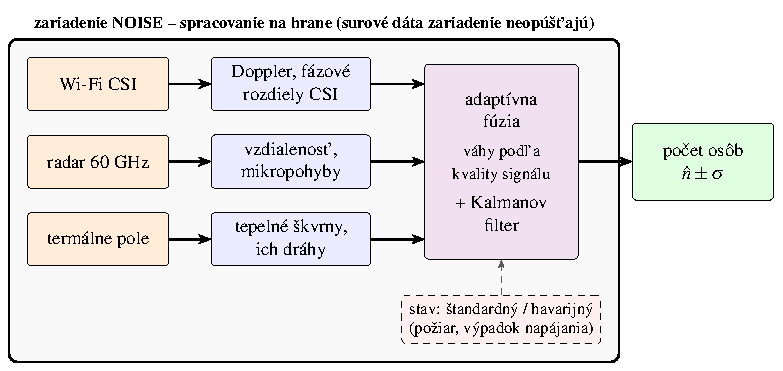
\includegraphics[width=0.9\textwidth]{architektura.pdf}
\caption{Architektúra spracovania v~module NOISE: tri nevizuálne modality, extrakcia príznakov, adaptívna fúzia a~anonymný výstup}\label{fig:architektura}
\end{figure*}

Modul obsahuje mikrokontrolér s~podporou zberu CSI, radar v~pásme 60~GHz a~termálne pole. Výber zodpovedá porovnaniu v~časti~\ref{porovnanie}: radar je najodolnejší a~zachytí dýchanie, termálne pole prináša presnosť pri malom počte osôb a~vysokú vrodenú anonymitu a~CSI je takmer bezplatným doplnkom. Z~každej modality sa extrahujú príznaky: z~CSI Dopplerovské spektrum a~fázové rozdiely~\cite{ma2019wifi}, z~radaru polohy odrazov a~mikropohyby vrátane dýchania~\cite{weiss2020people,hu2024mmcount}, z~termálneho poľa počet a~dráhy tepelných škvŕn, pričom statické zdroje tepla sa vylúčia podľa absencie mikropohybov~\cite{papanashi2026thermal}. Každá vetva poskytne vlastný odhad počtu osôb spolu s~mierou neistoty a~s~ukazovateľom kvality signálu -- napríklad kontrastom termálneho obrazu alebo stabilitou kanála.

Jadrom návrhu je \emph{adaptívna fúzia}. Váha každej vetvy sa mení podľa kvality jej signálu: keď kontrast termálneho poľa klesá, rozhodovanie sa presúva na rádiovú vetvu, keď je zarušená Wi-Fi, rozhoduje radar. Podobne ako pri váhovanej fúzii~\cite{rafi2024dwfl} má každá vetva svoju váhu, tú však chceme odvodzovať za behu z~ukazovateľov kvality signálu, aby systém reagoval aj na náhle zmeny, ako je zadymenie alebo vplyv ohňa na CSI~\cite{li2021fire}. Výsledný odhad sa časovo vyhladí Kalmanovým filtrom, aby krátkodobé výkyvy nespôsobovali skoky v~hlásenom počte. Výstupom je iba počet osôb s~intervalom neistoty; surové dáta zariadenie neopúšťajú (časť~\ref{sukromie}). Prispôsobenie novej miestnosti chceme riešiť doladením modelu z~malého počtu označených vzoriek, podobne ako pri metódach učenia z~malého počtu príkladov~\cite{hou2023dasecount}, keďže úplne bez údajov z~cieľového prostredia presnosť výrazne klesá~\cite{santos2024environment}.

Modul pracuje v~dvoch režimoch. V~\emph{štandardnom} režime je napájaný cez PoE, šetrí energiou a~zložitejšie modely spúšťa len pri zmene stavu; podobný princíp selektívneho vypínania modalít znížil spotrebu v~práci~\cite{cui2026em2}. Do \emph{havarijného} režimu prejde pri detekcii požiaru alebo výpadku napájania: beží na záložnej batérii, uprednostňuje radarovú vetvu a~detekciu dýchajúcich nehybných osôb a~častejšie odosiela svoj stav.

Merateľné ciele návrhu sme stanovili takto: v~miestnostiach do 15 osôb dosiahnuť odhad s~chybou najviac $\pm 1$ osoba v~aspoň 90\,\% meraní, v~zadymenej miestnosti zistiť prítomnosť nehybnej osoby do 30~sekúnd a~celý inferenčný reťazec vtesnať do pamäte mikrokontroléra s~nanajvýš 512~kB SRAM. Výsledky z~rešerše naznačujú, že ciele sú náročné, ale nie nereálne: presnosť $\pm 1$ osoba v~90--96\,\% prípadov dosiahli doteraz jednotlivé modality pri menšom počte osôb~\cite{korany2021stationary} a~spracovanie termálneho poľa sa už zmestilo do mikrokontroléra s~520~kB SRAM~\cite{papanashi2026thermal}; overiť treba najmä súčasný beh troch vetiev a~správanie pri 10--15~osobách.

% ---------------------------------------------------------------------
\section{Záver}\label{zaver}

Prehľad ukázal, že počet osôb v~miestnosti možno zisťovať bez kamier viacerými spôsobmi, no každý z~nich má iné slabiny: environmentálne senzory sú pomalé a~nepresné~\cite{chitnis2025environmental}, termálne polia strácajú kontrast pri vysokej teplote, Wi-Fi je citlivé na zmeny prostredia~\cite{santos2024environment} a~radar na prekrývanie odrazov~\cite{ren2023grouped}. Zároveň sme ukázali, že nevizuálne snímanie samo osebe nezaručuje anonymitu, lebo rádiové signály aj termálne obrazy nesú biometrické a~zdravotné informácie~\cite{wang2016gait,zhao2019mid,adib2015vital,yang2020muid,jiang2026warmgait} a~Wi-Fi kanál môže odpočúvať aj tretia strana~\cite{hernandez2021adversarial,xiao2025leakybeam}. Ochranu súkromia preto treba zabezpečiť architektúrou, konkrétne spracovaním priamo v~zariadení a~obmedzením toho, čo zariadenie vysiela.

Prínosom článku je zjednotenie dvoch pohľadov, ktoré sa v~literatúre objavujú oddelene, ochrany súkromia a~odolnosti v~krízových podmienkach, a~návrh konceptu NOISE, ktorý na ne odpovedá adaptívnou fúziou modalít. Otvorené zostávajú najmä tieto otázky: ako spoľahlivo odhadovať kvalitu jednotlivých signálov za behu, ako preniesť model do novej miestnosti bez zdĺhavej kalibrácie, ako sa presnosť správa pri rastúcom počte osôb, ako oheň a~horúce plyny ovplyvňujú rádiový kanál a~ako sa senzory skutočne správajú v~dyme a~pri vysokej teplote. Pre poslednú otázku sme v~rešerši nenašli verejný súbor údajov z~nevizuálnych senzorov s~počtom osôb v~zadymenej miestnosti; odpovede na ňu aj na ostatné otázky budeme hľadať meraním na prototype.

\bibliography{literatura}
\bibliographystyle{plain}

\end{document}
